\tikzstyle{terminal} = [rectangle, rounded corners, draw=black, fill=blue!30, inner sep=.2cm, text width=3.5cm, align=flush center]
\tikzstyle{others} = [rectangle, text centered, draw=black, inner sep=.2cm, align=flush center, text width=2.5cm]
\tikzstyle{arrow} = [draw, thick, ->, >=stealth]

\newcommand{\factorcolor}{red!30}
\newcommand{\externalcolor}{cyan!10}
\newcommand{\payoffcolor}{green!20}

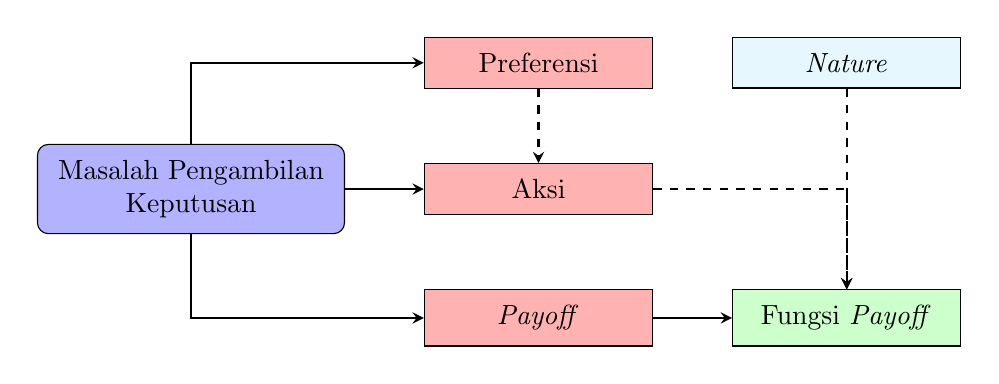
\begin{tikzpicture}[node distance=2cm]
  \matrix[column sep=1cm, row sep=7mm]{
                                                           & \node (pref) [others, fill=\factorcolor] {Preferensi};           &
    \node (nat) [others, fill=\externalcolor] {\textit{Nature}};                                                          \\
    \node (dp) [terminal] {Masalah Pengambilan Keputusan}; &
    \node (act) [others, fill=\factorcolor] {Aksi};        &                                                                    \\
                                                           & \node (po) [others, fill=\factorcolor] {\textit{Payoff}}; &
    \node (fpo) [others, fill=\payoffcolor] {Fungsi \textit{Payoff}};                                                    \\
  };

  \begin{scope}[every path/.style=arrow]
    \path (dp) -- (act);
    \path (dp) |- (pref);
    \path (dp) |- (po);
    \path (po) -- (fpo);
    \path [dashed] (pref) -- (act);
    \path [dashed] (act) -| (fpo);
    \path [dashed] (nat) -- (fpo);
  \end{scope}
\end{tikzpicture}